\documentclass[
  ngerman
  ,12pt
  ,pdftex
]{article}

\usepackage[utf8]{inputenc}
\usepackage{bericht}
\usepackage{framed}
\usepackage{graphicx}
\usepackage{blindtext}
\usepackage{setspace}
\usepackage{listings}
\usepackage{color}
\usepackage{hyperref}
\usepackage{lipsum}
\usepackage{cleveref}
\usepackage[printonlyused]{acronym}
\usepackage[center]{caption}
\usepackage{tocbibind}
\usepackage{titlesec}
\usepackage{xurl}
\usepackage{tocloft}                                              
\renewcommand\cftbeforetoctitleskip{-2cm}        % -> To fit TOC on one page

\definecolor{corange}       {rgb}{1.0,  0.52,   0.0}
\definecolor{clightblue}    {rgb}{0.0,  0.65,   1.0}
\definecolor{cpurple}       {rgb}{214,  0.37,   1.0}
\definecolor{cgreen}        {rgb}{0.0,  0.6,    0.08}
\definecolor{cdarkblue}     {rgb}{0.0,  0.29,   0.8}
\definecolor{cpink}         {rgb}{1.0,  0.0,    0.68}
\definecolor{clightgreen}   {rgb}{0.0,  1.0,    0.54}
\definecolor{cred}          {rgb}{0.8,  0.0,    0.0}
\definecolor{cyellow}       {rgb}{0.91, 0.89,   0.0}

\definecolor{arduinoGreen}    {rgb} {0.17, 0.43, 0.01}
\definecolor{arduinoGrey}     {rgb} {0.47, 0.47, 0.33}
\definecolor{arduinoOrange}   {rgb} {0.8 , 0.4 , 0   }
\definecolor{arduinoBlue}     {rgb} {0.01, 0.61, 0.98}
\definecolor{arduinoDarkBlue} {rgb} {0.0 , 0.2 , 0.5 }


\lstdefinelanguage{CSHARP}{
    language=[Sharp]C,
    %
    keywordstyle=\color{cdarkblue},     %%% Wörter der Sprache
    deletekeywords={Program, args, Console},
    morekeywords={class, string, @page, @model},
    %
    keywordstyle=[2]\color{cred},    %%% Namen, Namespaces
    keywords=[2]{Console, OnGetWeek, DateCheck, RedirectToPage},
    %
    keywordstyle=[3]\color{black},    %%% Standardwörter
    keywords=[3]{System},
    %
    keywordstyle=[4]\color{cgreen},  %%% Methoden, Funktionen
    keywords=[4]{Main, WriteLine, *ModelName*},
    %
    keywordstyle=[5]\color{clightblue},  %%% Variablennamen
    keywords=[5]{args, Program, console.log, DateTime},
    %
    stringstyle=\color{corange},
    commentstyle=\color{gray},
    %
    numbers=left,
    %
    breaklines=true,
    backgroundcolor=\color{gray!12!white},
    %
    showstringspaces=false,
    basicstyle=\ttfamily\small,
    captionpos=b,
    tabsize=2,
}
\lstdefinestyle{CSharp}{
    language=CSHARP,
    numbers=left,
    frame=single,
    xleftmargin=10pt,
}
\lstdefinestyle{CSharpBetween}{
    language=CSHARP,
    numbers=none,
    nolol,
}
%%%%%%%%%%%%%%%%%%%%%%%%%%%%%%%%%%%%%%%%%
\lstdefinelanguage{HypertextML}{
    language=html,
    %
    keywordstyle=\color{blue},     %%% Wörter der Sprache
    deletekeywords={class, id, value, href, html, charset, src, lang, rel, onclick},
    % otherkeywords={<, >, </},
    morekeywords={p, a, h1, h2, h3, h4, h5, body, head, div, canvas, span},
    %
    keywordstyle=[2]\color{black},    %%% Namen, Namespaces
    keywords=[2]{},
    %
    keywordstyle=[3]\color{black},    %%% Standardwörter
    keywords=[3]{},
    %
    keywordstyle=[4]\color{clightblue},  %%% Methoden, Funktionen
    keywords=[4]{onclick, html, charset, lang, rel, href},
    %
    keywordstyle=[5]\color{cgreen},  %%% Attribute
    keywords=[5]{class, id, src, alt},
    %
    stringstyle=\color{corange},
    commentstyle=\color{cgreen},
    %
    numbers=left,
    %
    breaklines=true,
    backgroundcolor=\color{gray!12!white},
    %
    showstringspaces=false,
    basicstyle=\ttfamily\small,
    captionpos=b,
    tabsize=2,
}
\lstdefinestyle{customHTML}{
    language=HypertextML,
    numbers=left,
    frame=single,
    xleftmargin=10pt,
}
\lstdefinestyle{HTMLBetween}{
    language=HypertextML,
    numbers=none,
    nolol,
}
%%%%%%%%%%%%%%%%%%%%%%%%%%%%%%%%%%%%%%%%%
\lstdefinelanguage{cshtml}{
    language=[Sharp]C,
    %
    alsoletter=-,
    keywordstyle=\color{blue},     %%% Wörter der Sprache
    deletekeywords={class, in, for},
    morekeywords={p, a, h1, h2, h3, h4, h5, body, head, html, div, canvas, span, ul, li, table, tr, td, input, label},
    %
    keywordstyle=[2]\color{cred},    %%% Namen, Namespaces
    keywords=[2]{@foreach, var, Console, in},
    %
    keywordstyle=[3]\color{clightblue},    %%% Standardwörter
    keywords=[3]{item, @item, set, @system, system, allSystems},
    %
    keywordstyle=[4]\color{clightblue},  %%% Methoden, Funktionen
    keywords=[4]{onclick},
    %
    keywordstyle=[5]\color{black},  %%% Attribute
    keywords=[5]{class, id, src, alt},
    %
    keywordstyle=[6]\color{cgreen},
    keywords=[6]{ToString, WriteLine, asp-page, asp-page-handler, method, @TSDTestSystemsDynamic},
    %
    stringstyle=\color{corange},
    commentstyle=\color{gray},
    %
    numbers=left,
    %
    breaklines=true,
    backgroundcolor=\color{gray!12!white},
    %
    showstringspaces=false,
    basicstyle=\ttfamily\small,
    captionpos=b,
    tabsize=2,
}
\lstdefinestyle{CSHTMl}{
    language=cshtml,
    numbers=left,
    frame=single,
    xleftmargin=10pt,
}
\lstdefinestyle{CSHTMLBetween}{
    language=cshtml,
    numbers=none,
    nolol,
}
%%%%%%%%%%%%%%%%%%%%%%%%%%%%%%%%%%%%%%%%%%
\lstdefinelanguage{css}{
    alsoletter={., \#, -},
    keywordstyle=[1]\color{cdarkblue},
    keywords=[1]{.myClass1, .myClass2, p, a},
    %
    keywordstyle=[2]\color{clightblue},
    keywords=[2]{color, background-color, transform},
    %
    keywordstyle=[3]\color{corange},
    keywords=[3]{},
    %
    stringstyle=\color{corange},
    commentstyle=\color{cgreen},
    morecomment=[s]{/*}{*/},
    %
    numbers=left,
    %
    breaklines=true,
    backgroundcolor=\color{gray!12!white},
    %
    showstringspaces=false,
    basicstyle=\ttfamily\small,
    captionpos=b,
}
\lstdefinestyle{CSS}{
    language=css,
    numbers=left,
    frame=single,
    xleftmargin=10pt,
}
%%%%%%%%%%%%%%%%%%%%%%%%%%%%%%%%%%%%%%%%%%
\lstdefinelanguage{js}{
    language=[Sharp]C,
    %
    alsoletter={'},
    keywordstyle=\color{cdarkblue},     %%% Wörter der Sprache
    deletekeywords={Program, args, Console, const, var, let},
    morekeywords={class, string},
    %
    keywordstyle=[1]\color{clightblue},  %%% Methoden, Funktionen
    keywords=[1]{addEventListener, getElementById, log},
    %
    keywordstyle=[2]\color{blue},  %%% Methoden, Funktionen
    keywords=[2]{console, const, var, let, document},
    %
    keywordstyle=[3]\color{cred},  %%% Methoden, Funktionen
    keywords=[3]{'click'},
    %
    stringstyle=\color{black},
    commentstyle=\color{gray},
    %
    numbers=left,
    %
    breaklines=true,
    backgroundcolor=\color{gray!12!white},
    %
    showstringspaces=false,
    basicstyle=\ttfamily\small,
    captionpos=b,
    tabsize=2,
}
\lstdefinestyle{JavaScript}{
    language=js,
    numbers=left,
    frame=single,
    xleftmargin=10pt,
}



\newcommand{\Autor}{Niklas Rodenbüsch}
\newcommand{\MatrikelNummer}{6130555}
\newcommand{\Kursbezeichnung}{TINF21B4}

\newcommand{\FirmenName}{SICK AG}
\newcommand{\FirmenStadt}{Waldkirch}
% Falls es kein Firmenlogo gibt:
\newcommand{\FirmenLogoDeckblatt}{
\includegraphics[width=3cm]{images/SICK_Logo.jpg}}

\newcommand{\BetreuerFirma}{Tobias Weckerle, MBA}
\newcommand{\BetreuerDHBW}{Mirko Dostmann}

%%%%%%%%%%%%%%%%%%%%%%%%%%%%%%%%%%%%%%%%%%%%%%%%%%%%%%%%%%%%%%%%%%%%%%%%%%%%%%%%%%%%%

\newcommand{\Was}{Finanzmanager}

%%%%%%%%%%%%%%%%%%%%%%%%%%%%%%%%%%%%%%%%%%%%%%%%%%%%%%%%%%%%%%%%%%%%%%%%%%%%%%%%%%%%%

\newcommand{\Titel}{Advanced Software-Engineering Programmentwurf}
\newcommand{\AbgabeDatum}{10.05.2024}

\newcommand{\Dauer}{5. \& 6. Semester}

\newcommand{\Abschluss}{Bachelor of Science}

\newcommand{\Studiengang}{Informatik / Angewandte Informatik}

\def\figureautorefname{\acs{abb}}
\renewcommand{\lstlistingname}{Quellcode}
\renewcommand{\lstlistlistingname}{Liste der Quellcodes}

\begin{document}

\newcommand{\q}[1]{{\glqq #1\grqq{}}}
\newcommand{\cf}[1]{\cite[vgl.][]{#1}}

\pagestyle{fancy}
\fancyhf{}
\fancyhead[L]{\rightmark}
\fancyfoot[C]{\thepage}
\renewcommand{\headrulewidth}{0.4pt}

%%%%%%%%%%%%%%%%%%%%%%%%%%%%%%%%%%%%%%%%%%%%%%%%%%%%%%%%%%%%%%%%%%%%%%%%%%%%%%%

\begin{titlepage}
    \begin{center}
        \vspace*{-2cm}
        \FirmenLogoDeckblatt\hfill
\includegraphics[width=4cm]{images/dhbw-logo}\\[2cm]
        {\Huge \Titel}\\[1cm]
        {\Huge\scshape \Was}\\[1cm]
        {\large für die Prüfung zum}\\[0.5cm]
        {\Large \Abschluss}\\[0.5cm]
        {\large des Studienganges \Studiengang}\\[0.5cm]
        {\large an der}\\[0.5cm]
        {\large Dualen Hochschule Baden-Württemberg Karlsruhe}\\[0.5cm]
        {\large von}\\[0.5cm]
        {\large\bfseries \Autor}\\[1cm]
        % {\large Abgabedatum \AbgabeDatum}
        \vfill
    \end{center}
    \begin{tabular}{l@{\hspace{2cm}} l}
        Bearbeitungszeitraum          & \Dauer           \\
        Matrikelnummer                & \MatrikelNummer  \\
        Kurs                          & \Kursbezeichnung \\
        Gutachter der Studienakademie & \BetreuerDHBW    \\
    \end{tabular}\\[1cm]
    \begin{tabular}{l}
        Reposiory: \url{https://github.com/NI-R0/DH-Software-Engineering-II} \\
    \end{tabular}
\end{titlepage}

%%%%%%%%%%%%%%%%%%%%%%%%%%%%%%%%%%%%%%%%%%%%%%%%%%%%%%%%%%%%%%%%%%%%%%%%%%%%%%%
\begin{onehalfspace}

    %%%%%%%%%%%%%%%%%%%%%%%%%%%%%%%%%%%%%%%%%%%%%%%%%%%%%%%%%%%%%%%%%%%%%%%%%%%%%%%

    \newpage
    \pagenumbering{Roman}
    \tableofcontents

    \newpage
    \newcounter{savepage}
    \setcounter{savepage}{\value{page}}
    \pagenumbering{arabic}

    %%%%%%%%%%%%%%%%%%%%%%%%%%%%%%%%%%%%%%%

    % Jetzt kommt der "eigentliche" Text
    
    \chapter{Domain Driven Design}
\section{Analyse der Ubiquitous Language}

Die Ubiquitous Language des Projektes richtet sich nach der üblichen Sprache der Domäne \q{Finanzsektor}. Die im Folgenden erläuterten Begriffe sind speziell aus der Subdomäne \q{Finanzverwaltung} entnommen und werden im weiteren Verlauf des Projektes verwendet.

\paragraph*{\q{Konto} (Account):} Der Begriff bezeichnet eine Einheit, in der finanzielle Transaktionen abgewickelt werden können. Es gibt zwei verschiedene Arten von Konten: Bankkonten und Investmentkonten.

\paragraph*{\q{Bankkonto} (Bank account):} Ein Bankkonto ist ein Konto, das für alltägliche Finanztransaktionen wie Einnahmen und Ausgaben genutzt wird. Es gehört zu einer bestimmten Bank und hat einen eindeutigen Namen.

\paragraph*{\q{Investmentkonto} (Investment account):}  Ein Investmentkonto ist ein Konto, das für den Kauf und Verkauf von Vermögenswerten genutzt wird. Es gehört zu einem bestimmten Broker und hat ebenfalls einen eindeutigen Namen.

\paragraph*{\q{Transaktion} (Transaction):} Transaktionen sind Ereignisse, die eine Veränderung des Kontostandes verursachen. Dazu gehören Einnahmen, Ausgaben, sowie Käufe und Verkäufe von Vermögenswerten. Transaktionen gehören immer zu genau einem Konto.

\paragraph*{\q{Vermögenswert} (Asset):} Ein Vermögenswert ist eine Ressource, die einen monetären Wert besitzt und von Benutzern gehandelt werden kann, mit der Absicht, finanzielle Gewinne oder langfristige Wertsteigerungen zu erzielen. Vermögenswerte können verschiedene Formen wie Aktien, Fonds, Rohstoffe oder Kryptowährungen annehmen.

\paragraph*{\q{Einnahme} (Income):} Einnahmen sind finanzielle Zuflüsse auf ein Bankkonto, die den Kontostand erhöhen.

\paragraph*{\q{Ausgabe} (Expense):} Ausgaben sind finanzielle Abflüsse von einem Bankkonto, die den Kontostand verringern.

\paragraph*{\q{Kauf/Verkauf von Vermögenswerten} (Purchase/Sale of Assets):} Diese Form von Transaktionen bezieht sich auf den Kauf, bzw. Verkauf von Vermögenswerten.

\paragraph*{\q{Broker}:} Ein Broker ist eine Organisation, die als Vermittler für den Kauf und Verkauf von Vermögenswerten fungiert.

\paragraph*{\q{Bank}:} Eine Bank ist eine finanzielle Institution, die Dienstleistungen wie z.B. die Verwaltung von Bankkonten, Kreditvergaben, usw. anbietet.

\paragraph*{\q{Kontostand} (Balance):} Der Kontostand ist der aktuelle Geldbetrag, der auf einem Konto verfügbar ist. Er errechnet sich aus der Summe aller durchgeführten Transaktionen und kann sowohl positive als auch negative Zahlen annehmen.

\paragraph*{\q{Benutzer} (User):} Der Benutzer der Anwendung, der die Konten erstellt und Transaktionen durchführt.









%%%%%%%%%%%%%%%%%%%%%%%%%%%%%%%%%%%%%%%%%%%%%%%%%%%%%%%
\section{Analyse und Begründung der verwendeten Muster}
Value Objects, Entities, Aggregates, Repositories, Domain Services

    \chapter{Clean Architecture}
Aufgabe: Schichtarchitektur planen und begründen\\

Abhängigkeiten nur von innen nach außen\\
4. Abtraction (Abstraktionen, nicht unbedingt nötig, ändert sich nie)\\
3. Domain (DDD Code: Aggregates, Entities, Values)\\
2. Application (Enthält Application Use-Cases (nicht Domain use cases))\\
1. Adapters (Daten-Tausch-Objekte)\\
0. Plugins (DB/GUI/..., arbeitet nur mit Adaptern)


    \chapter{Programming Principles}
%Aufgabe: Analyse und Begründung für 5 der vorgestellten Prinzipien (SOLID/GRASP/DRY/KISS/YAGNI/Conway)
\section{Dependency Inversion Principle}
\label{chap:dip}
Das Dependency Inversion Principle (kurz: DIP) besagt, dass Module hoher Ebenen nicht von Modulen niedriger Ebenenen abhängen sollten. Stattdessen sollten beide von Abstraktionen abhängen. Weiterhin sollten Abstraktionen nicht von Details abhängen, sondern umgekehrt.\\
Ein Beispiel hierfür sind die ApplicationServices, deren einzige Abhängigkeit zur Domain-Schicht in der Verknüpfung mit dem entsprechenden Domain-Repository-Interface (also der Abstraktion des Repositories) liegt. Die eigentliche Verknüpfung erfolgt zur Laufzeit über eine Injection durch die @Autowired-Annotation von Spring Boot.
\vspace*{0.5cm}
\begin{figure}[!htb]
    \centering{
        
\includegraphics[width=14cm]{images/dip.png}}
    \caption[Dependency Inversion Principle]{DIP-Beispiel anhand der Klasse InstitutionApplicationService}
    \label{fig:dip}
\end{figure}

\section{Low Coupling}
Der Begriff \q{Kopplung} gilt als Maß für die Abhängigkeit einer Klasse von ihrer Umgebung. Das Prinzip \q{Low Coupling} besagt also, dass die Kopplung von Klassen so niedrig wie möglich gehalten werden sollte. Ein Beispiel aus der Anwendung ist die Persistence-Schicht. Die einzigen Klassen, die direkt mit dieser Schicht zusammenarbeiten, sind die \q{RepositoryBridges} Persistence-Schicht. Somit könnte beispielsweise die Datenbank ausgetauscht werden, ohne dafür große Teile der Anwendung ändern zu müssen.

\section{High Cohesion}
Hohe Kohäsion ist ein Maß für den inneren Zusammenhalt einer Klasse, also wie \q{eng} Methoden und Attribute einer Klasse zusammenarbeiten. Dieses Prinzip wurde beispielsweise durch die Implementierung des ValueObjects \q{AccountOwnerNameValue} berücksichtigt, das den Namen eines Account Besitzers enthält. Da der Name eines Account Besitzers an sich nichts mit den anderen Eigenschaften eines Accounts zu tun hat, erhöht die Einführung des ValueObjects die Kohäsion.
%ValueObject

\section{Indirection}
Das Prinzip \q{Indirection} bezeichnet das Delegieren von Aufgaben an andere Objekte und Klassen. Ein Beispiel aus der Anwendung hierfür sind die Methoden der Domain-Repositories (siehe Abb. \ref{fig:indirection}) die ihre eigentlichen Aufgaben lediglich an die JPA-Repositories weitergeben.

\section{Controller}
Der Controller ist das erste Objekt hinter der UI, das Anweisungen annimmt und kontrolliert. Er ist quasi die \q{Steuereinheit} des Programms. Der Controller ist in der Regel der einzige Ansprechpartner, den die UI hat. Er empfängt dabei Anweisungen von der UI und delegiert diese, ohne viel eigene Funktionalität zu implementieren, an Domain-Objekte und Services weiter.\\
Beispiele für Controller in der Anwendung sind die REST-Controller-Klassen der API-Schicht.

\begin{figure}[!htb]
    \centering{
        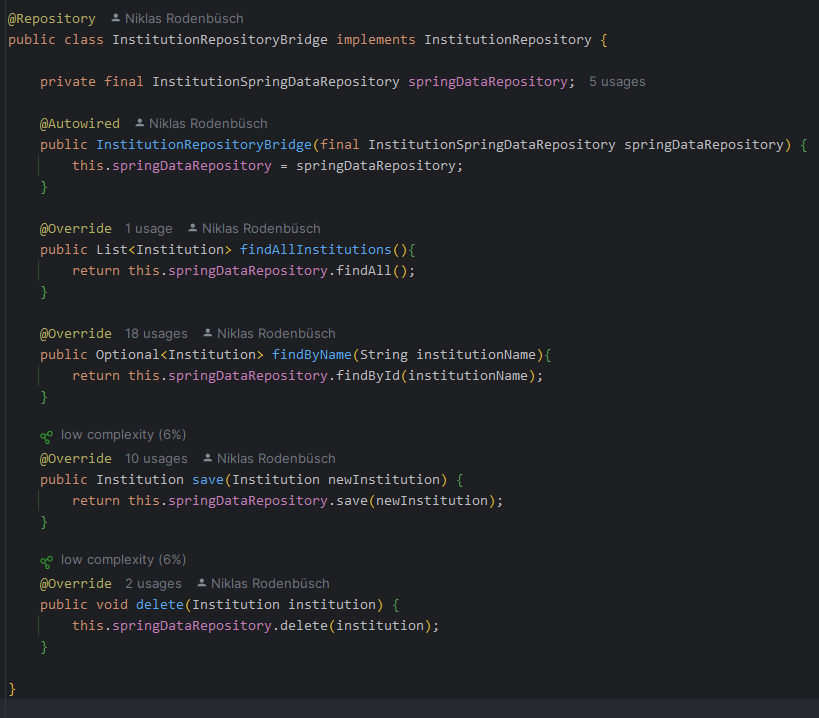
\includegraphics[width=16.5cm]{images/indirection.png}}
    \caption[Indirection Principle]{Indirection principle anhand der Klasse InstitutionRepositoryBridge}
    \label{fig:indirection}
\end{figure}

    \chapter{Refactoring}
Code smells identifizieren und die Durchführung von mindestens zwei Refactorings begründen.

    Einsatz von Entwurfsmustern ausführlich begründen.

    %%%%%%%%%%%%%%%%%%%%%%%%%%%%%%%%%%%%%%%

    \newpage
    \pagenumbering{Roman}
    \setcounter{page}{\value{savepage}}


    % \chapter*{Abkürzungsverzeichnis}
    % \addcontentsline{toc}{chapter}{Abkürzungsverzeichnis}
    % \begin{acronym}[AAAAAA]
    \acro{dat}[DAT]{Dezentrales Analysetool}
    \acro{tsd}[TSD]{Testsystemdatenbank}
    \acro{sdat}[smartDAT]{Smarten Dezentralen Analysetool}
    \acro{html}[HTML]{Hypertext Markup Language}
    \acro{css}[CSS]{Cascading Style Sheets}
    \acro{js}[JS]{JavaScript}
    \acro{abb}[Abb.]{Abbildung}
    \acro{s}[S.]{Seite}
    \acro{gbc}[GBC]{Global Business Center}
    \acro{bu}[BU]{Business Unit}
    \acro{sick}[SICK]{SICK AG}
    \acro{zb}[z.B.]{zum Beispiel}
    \acro{mrd}[Mrd.]{Milliarden}
    \acro{sbf}[SBF]{Smart Button Factory}
    \acro{cd}[CD]{Corporate Department}
    \acro{cu}[CU]{Corporate Unit}
    \acro{it}[IT]{Information Technology}
    \acro{ssc}[SSC]{Sales and Service Cluster}
    \acro{ssu}[SSU]{Sales and Service Unit}
    \acro{gic}[GIC]{Global Industry Center}
    \acro{fdt}[FDT]{Fault Diagnostics Tool}
    \acro{api}[API]{Application Programming Interface}
    \acro{lts}[LTS]{Langzeitsupport}
    \acro{iot}[IOT]{Internet of Things}
    \acro{dom}[DOM]{Document Object Model}
    \acro{json}[JSON]{JavaScript Object Notation}
    \acro{api}[API]{Application Programming Interface}

\end{acronym}
    % \newpage

    %%%%%%%%%%%%%%%%%%%%%%%%%%%%%%%%%%%%%%%

    % \listoffigures
    % \newpage

    % \lstlistoflistings

    %%%%%%%%%%%%%%%%%%%%%%%%%%%%%%%%%%%%%%%

    % \newpage
    % \def\refname{Literaturverzeichnis}        % -- Einträge in test_bib.bib
    % \nocite{*}
    % \addcontentsline{toc}{chapter}{Literaturverzeichnis}
    % \printbibliography

    %%%%%%%%%%%%%%%%%%%%%%%%%%%%%%%%%%%%%%%

\end{onehalfspace}
\end{document}